\chapter{Integrace do průmyslu 4.0}
Pojem Průmysl 4.0 se do České republiky dostal okolo roku 2013 a od té doby se stále více rozšiřuje v průmyslových firmách.
Jedna z klíčových částí je IoT (Internet of Things), neboli v internet věcí, který nám zajišťuje vzdálenou kontrolu a řízení strojů pomocí elektroniky, senzorů a různých softwarů.
Další vlastností těchto systémů je zaznamenávání a následné ukládání dat do datových úložišť.
Moderní IoT řídící systémy se snaží proniknou co nejvíce do hloubky řídících systém a zpřesnit tak naměřená data, důležitá pro optimalizaci produkce.   

\section{Popis}
Při návrhu mého systému jsem se snažil řídit těmito zásadami a navrhnout tak co nejmodernější a~provozně efektivní systém.
Základem bylo zhodnocení stávající situace a~navržení možného řešení.

Jedntlivé problémy
\begin{itemize}
    \item dlouhá doba stání nečinných strojů
    \item ruční počítání vyprodukovaného zboží
    \item absence historického přehledu produkce
\end{itemize}

\section{Řešení}
Mým řešením je tedy návrh moderního systému, který by celý tento provoz monitoroval a zobrazoval zaměstnavateli.
Dále se také snažím o zhodnocení jednotlivých směn a~jejich porovnání.
% Systém je neustále vyvíjen a rozšiřován o nové funkcionality navržené firmou.
Systém neustále vyvíjím a~rozšiřuji podle potřeb firmy.

%SECTION
\section{Naszaení}
Jak jsem již psal, tento systém je aktuálně nasazen ve firmě ROTEX Vysočina s.r.o\cite{ROTEX}, která se věnuje výrobou ponožek. 
Firma pracuje ve dvousměnném provozu a~týdně vyprodukuje v~průměru 12000 párů ponožek. 

Díky mému systémy by se ve firmě dala optimalizovat produkce a~výkon strojů a~tím zefektivnit budoucí výrobu. 

\begin{figure}[htbp]
    \centering
    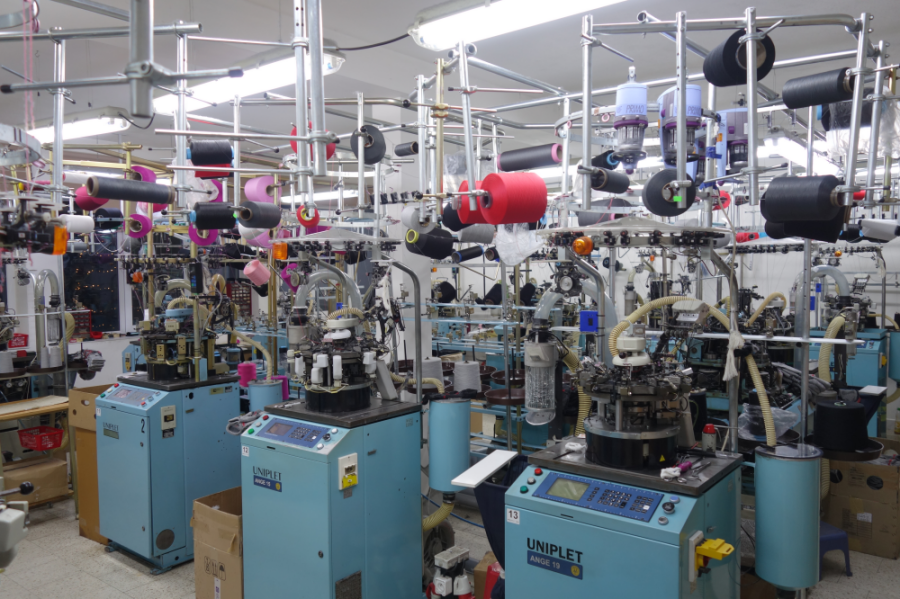
\includegraphics[width=\textwidth]{img/pletarna.png}
    \caption{Pletárna ponožek}
    \label{fig:Pletarna}
\end{figure}

\begin{figure}[htbp]
    \centering
    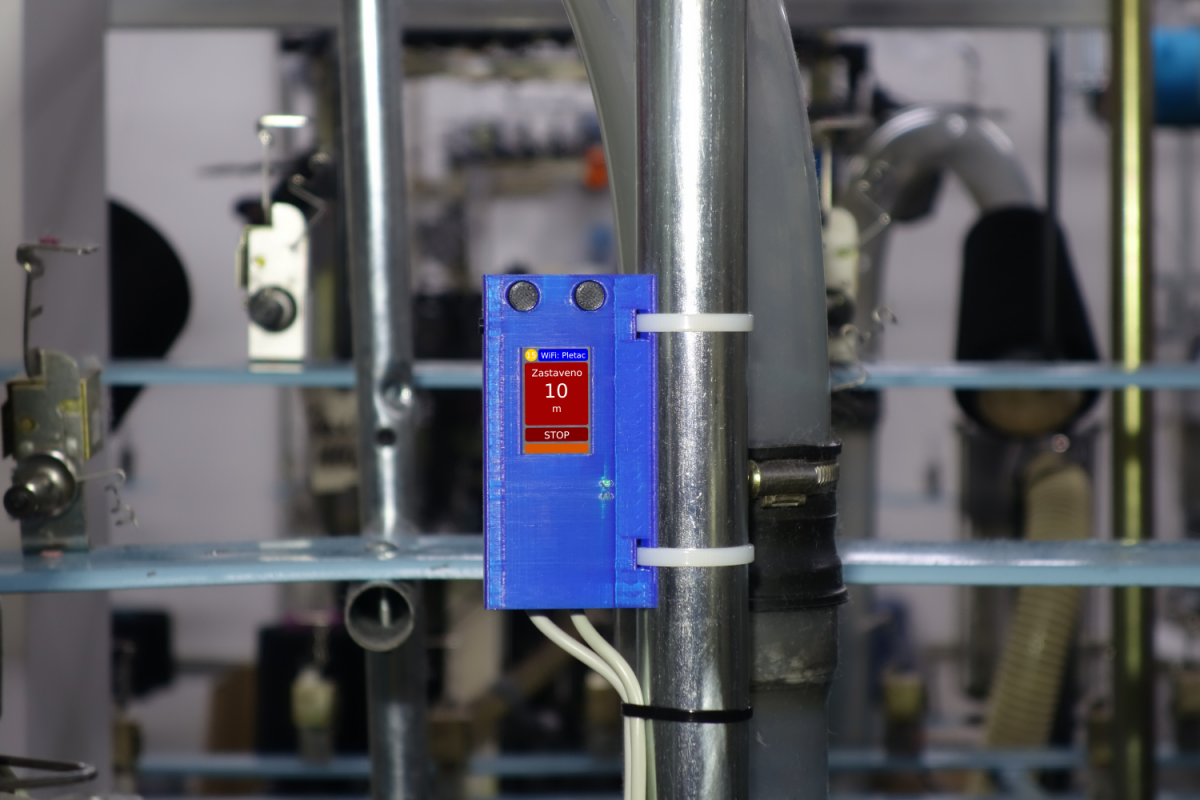
\includegraphics[width=\textwidth]{img/V2-uchyceni-stop.png}
    \caption{Senzor na stroji}
    \label{fig:SenzorNaStroji}
\end{figure}


\newpage